\documentclass[12pt]{report}
\usepackage[utf8]{inputenc}
\usepackage[T1]{fontenc}

\usepackage{extramarks}
\usepackage{fancyhdr}
\usepackage{graphicx}
\usepackage[margin=25mm]{geometry}
\usepackage{tikz}
\usepackage{float}
\usepackage{longtable}
\usepackage{amsmath}
\usepackage{caption}

% "Less is more" chapter formatting
\usepackage{titlesec, color}
\definecolor{gray75}{gray}{0.75}
\newcommand{\hsp}{\hspace{20pt}}
\titleformat{\chapter}[hang]{\Huge\bfseries}{\thechapter\hsp\textcolor{gray75}{|}\hsp}{0pt}{\Huge\bfseries}

\usepackage[style=ieee,backend=biber]{biblatex}
\bibliography{references.bib}

\pagestyle{fancy}
\setlength{\headheight}{14.5pt}
\lhead{Build a Better Wheelchair: Project Report}
\rhead{The FoWheel Team}
\cfoot{\thepage}

\title{
\includegraphics[width=25mm]{minesbw}\vspace{10 mm}\\Build a Better Wheelchair:
Project Report \vspace{20mm}\\}
\author{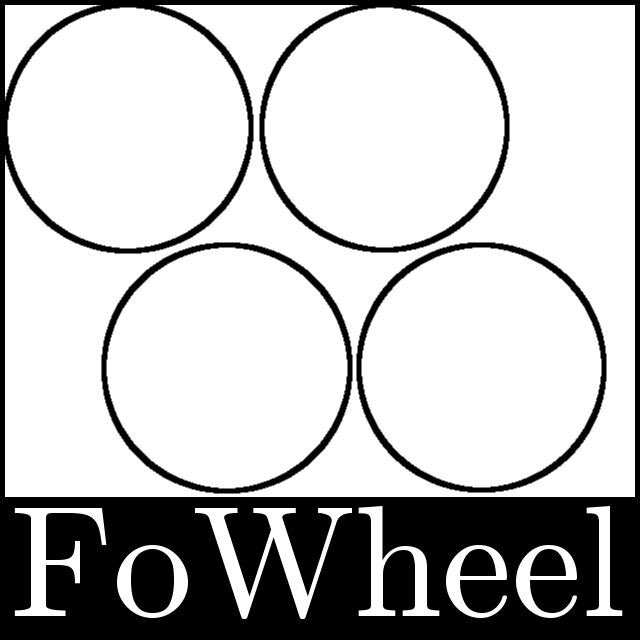
\includegraphics[width=25mm]{fowheellogo}\vspace{10 mm}\\Colorado School of Mines, The FoWheel Team, Section M\&N
\vspace{6 pt} \\
\begin{tabular}[h!]{c c}
    Jack Rosenthal & Joseph Bales \\[2pt]
    \texttt{jrosenth@mines.edu} & \texttt{jbales@mines.edu}
\end{tabular} \vspace{12 pt}
\\
\begin{tabular}[h!]{c c c}
    Ilman Surghani & Robert Schreibman & Arbnol Sopaj \\[2pt]
    \texttt{isurghan@mines.edu} & \texttt{rschreib@mines.edu} & \texttt{asopaj@mines.edu}
\end{tabular}
}
\date{17 April 2015}

\renewcommand{\arraystretch}{1.5}
\setlength{\parindent}{0mm}
\setlength{\parskip}{6pt plus1pt minus1pt}

\usetikzlibrary{math}

%\tikzmath{
%    function FordCircles(\a,\b,\n){
%        int \p, \q; % ------------------------------ p and q are integers
%        for \q in {1,...,\n}{ % -------------------- 0 < q <= n
%            for \p in {\a*\q,...,\b*\q}{ % ----------- a < p/q < b <=> [aq] < p < [bq]
%                if gcd(\p,\q) == 1 then { % ------------ if the fraction is irreducible
%                    \f = \p/\q; % ------------------------ evaluate the tuch point f = p/q
%                    \r = 1/(2*\q*\q); % ------------------ evaluate the radius r = 1/2q^2
%                    {
%                        \draw[black] (\f,\r) circle(\r); % --- and draw the Ford circle at (f,r)
%                    };
%                };
%            };
%        };
%    };
%}

\begin{document}

\pagestyle{empty}

%\begin{minipage}{\textwidth}
%    \begin{flushright}
%        \hfill \vspace{10mm} \\
%        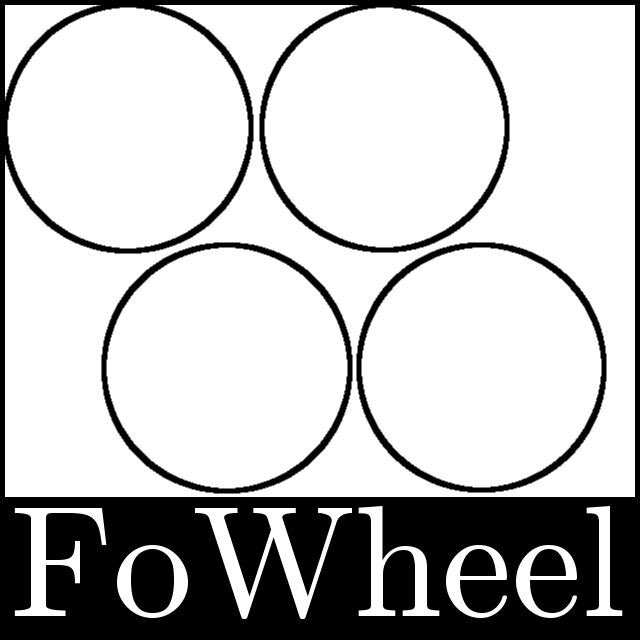
\includegraphics[height=48pt]{fowheellogo}
%        \parbox{3cm}{Team FoWheel \\ Spring 2015 \\ EPICS 151 \\ Section M\&N}
%    \end{flushright}
%\end{minipage}

\hfill \vspace{10mm} \\

    \begin{flushright}
\begin{tabular}{l l}
    \parbox{49pt}{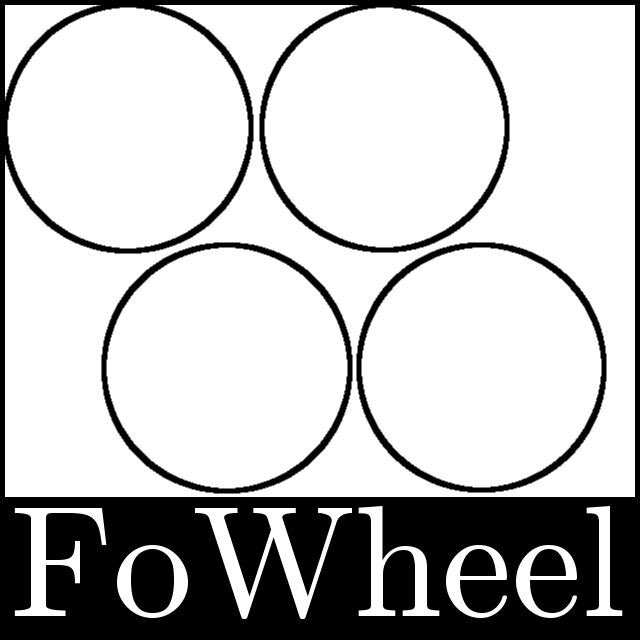
\includegraphics[height=48pt]{fowheellogo}} & \parbox{3cm}{Team FoWheel \\
Spring 2015 \\ EPICS-151 \\ Section M\&N}
\end{tabular}
    \end{flushright}

\begin{minipage}{\textwidth}
Crutches 4 Africa \\
284 S. Franklin St. \\
Denver, Colorado 80209 USA
\end{minipage}

17 April 2015

Dear Mr. Talbot,

Attached is the report for Team FoWheel's response to your Build a Better
Wheelchair project. This report is based on the hazards encountered by
wheelchair users in Africa and addresses those hazards to the fullest extent
possible. FoWheel was assigned this project on 7 January 2015.

This report explains the process FoWheel used to design a more effective
wheelchair. Several ideas were conceived as to upgrades which could be applied
to the basic wheelchair design. Through a decision matrix, we selected three
modifications we could make. Each of these modifications was dubbed a subsystem
and further analyzed. This analysis included material and cost breakdowns. Our
three modifications address three distinct problems: traction, safety, and
carrying objects.

Our assembly instructions have been drawn rather than written in the hopes that
they can be sent to workers with limited or no English vocabulary without much
revising. The rest of the report, however, is meant for you and your evaluation
of the design.

It has been an honor working on a project which could improve so many lives. We
hope that our design makes a difference.

Best Wishes,

Team FoWheel

\pagenumbering{roman}
\clearpage
\maketitle

\chapter{Executive Summary}

While wheelchairs may be common or in excess in the United States
and other developed countries, wheelchairs and many other mobility devices are
less common in rural locations in Africa. According to Disability Network
Africa, one in four people have a mobility disability in rural communities, and
most of which are in need of a mobility device\cite{dna-disabled}. Additionally, standard
wheelchairs which are discarded in developed countries are unsuitable for the
variable terrain in Africa.

The FoWheel team has been tasked with implementing a wheelchair modification
process to improve donated wheelchair usability in rural African communities.
Our team identified three main flaws with current donated wheelchairs:
lack of traction, risk of falling out, and carrying liquids or supplies while simultaneously
powering the chair. To address these issues, team FoWheel has
implemented three modifications to the current donated wheelchairs' design: the
addition of mountain bike tires, a seatbelt, and a cup holder.

To address the issue of traction, our team has added mountain bike tires
to our design. These mountain bike tires wrap around the original wheelchair
wheels. The tires can be removed from old bicycles, or are available at low
cost.

To allow the user to carry cups or other small objects, our team has implemented a foam cup
holder in our design. The foam cup holder is removable, making the addition a
versatile modification. The cup holder is a low cost addition of only cents per
wheelchair.

To prevent the user from falling out of the wheelchair, and additionally
provide the ability to carry a variety of larger items, our design implements a
seatbelt. The seatbelt secures the user in the chair and attaches in a diagonal fashion similar
to car seatbelts. The user can secure larger items in their lap with the
seatbelt, making this modification multipurpose. The seatbelt costs only 0.70
USD per chair.

As the assemblers of this project may not be fluent in English, this report
contains illustrated installation instructions in addition to written
instructions for each of our modifications.

As Crutches4Africa is a non-profit organization, our team's primary goal in
our design was to keep the cost low. The total design costs a maximum of only
13.22 USD per wheelchair. Our cost estimate is under the assumption that modifications will
be preformed by volunteers; however, this cost includes all materials should
they need to be purchased. These retrofits not only solve all aforementioned
problems, but together are under the suggested budget of 50 USD and can be more
effective than many commercial solutions.
\clearpage

\tableofcontents
\begin{minipage}{\textwidth}
\listoffigures
\end{minipage}
\begin{minipage}{\textwidth}
\listoftables
\end{minipage}

\pagestyle{fancy}

\chapter{Introduction}
\pagenumbering{arabic}

In January of 2015, the FoWheel team was presented with a project by
Crutches4Africa. Current donated wheelchairs brought to local communities in
Africa are unsuitable for use in rough terrain, and do not meet the needs of
the users, caregivers, and other involved stakeholders. Team FoWheel brings a
design based off of retrofitting donated wheelchairs to better meet the needs
of the stakeholders.

The purpose of this report is to explain how to implement team FoWheel’s
retrofit designs onto wheelchairs. Additionally, this report explains the team's
thought processes behind our design, and analyzes the effectiveness in
correcting bugs found with current wheelchairs used in rural Africa.

\section{Background Information}
The earliest wheelchair design that resembles modern day wheelchairs was
invented in 1919, by Herbert Everest\cite{everest-wheelchair}. Everest was a mining engineer who
invented the modern wheelchair after breaking his back in a mining
accident\cite{everest-wheelchair}. This was the first automobile
friendly design with a fold-up feature that made the chair compact and
portable. Wheelchairs have brought mobility to many since then; however, some rural communities in Africa
have only recently started to receive mobility devices. Additionally, the rough
terrain in many areas makes wheelchairs impractical. Various off-road and
all-terrain wheelchairs have been invented and are commercially available in
developed countries\cite{oxford1992all}\cite{wilmot2007off}\cite{wilmot2011off}. These off-road wheelchairs are expensive
however, and unavailable to the communities that need them in Africa.

\section{Design Alternatives and Selection Process}
Our design was chosen using
a decision matrix that evaluated the adaptations based on overall
usefulness, practicality, and cost. The decision matrix, as seen in
Figure~\ref{fig:decision-matrix} shows our process in selecting our design. We
also selected a secondary design, also seen in the matrix.

\begin{figure}
    \centering
    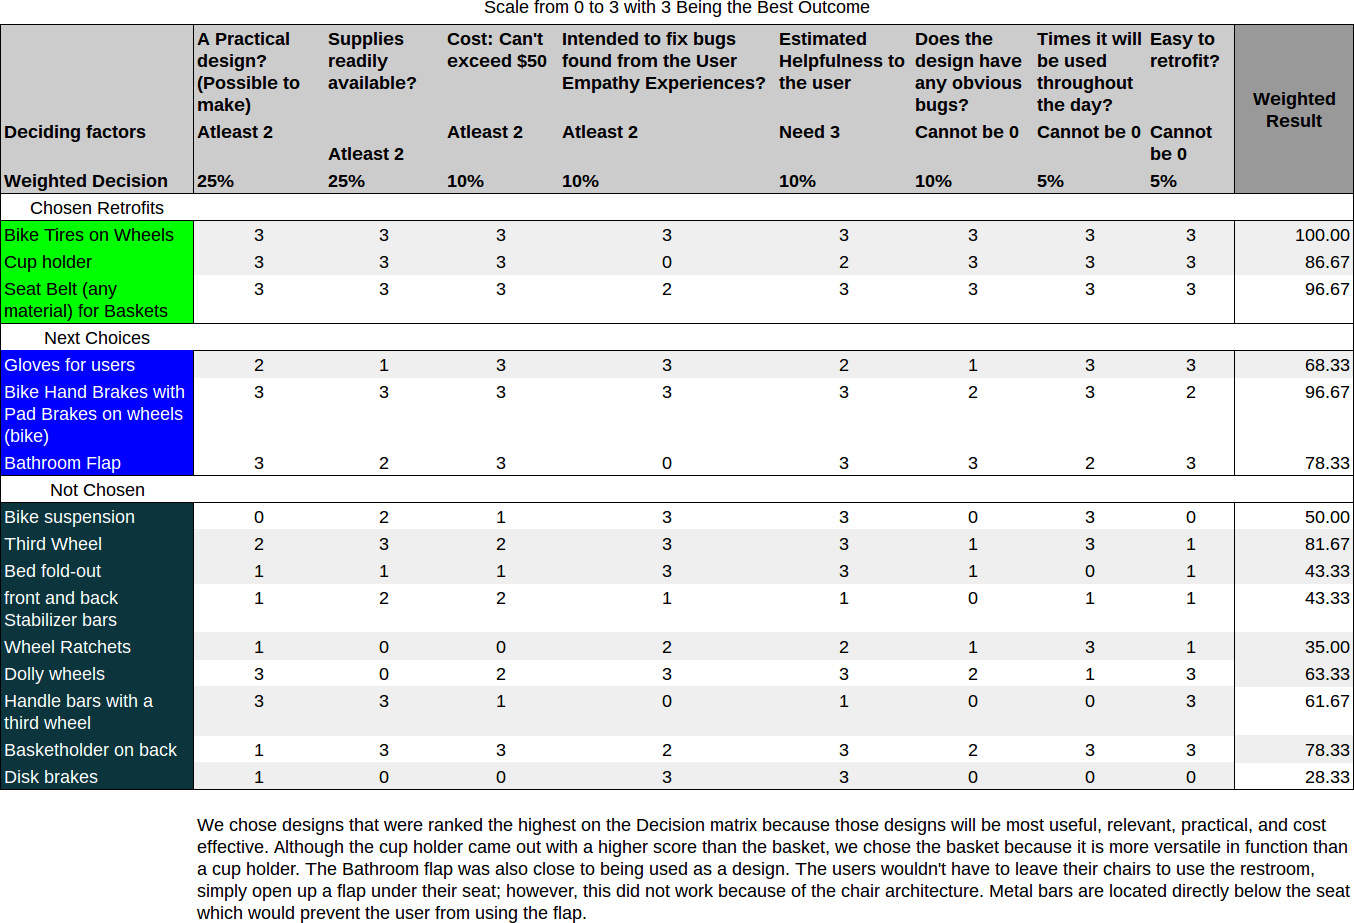
\includegraphics[width=0.9\textwidth]{decision-matrix}
    \caption{The Decision Matrix}
    \label{fig:decision-matrix}
\end{figure}

Our design implementation emphasizes using readily
available materials in local communities in Africa that are either recycled or of low cost.
As some local communities in Africa have a limited availability
of tools, all of our adaptations are able to be retrofitted with simple tools
such as a screwdriver and an adjustable wrench.

The primary stakeholder for this project is the end user. Our team identified the major problems faced
by the end user as:

\begin{itemize}
    \item Slipping when rotating the wheels on low friction
        surfaces
    \item Difficulty carrying objects when the hands are occupied rotating the wheels
    \item Falling out of the wheelchair
    %\item Injuring hands when slowing or stopping the wheels
\end{itemize}

\section{Proposed Solution}

To properly address these problems, our team created three subsystems within
our wheelchair retrofit design. These subsystems are:

\begin{itemize}
    \item Mountain bike tires to provide better ground traction
    \item A safety strap to prevent the user from falling out of their
        wheelchair, that can additionally be tied to large objects to carry
    \item A cup holder that can be used to carry water or smaller objects
\end{itemize}

%In addition to these three subsystems, our design implementation recommends the
%use of low cost gloves for braking.
%Our team decided to implement brakes using gloves rather the installation of
%existing bicycle brakes due to the costs and complexity bike brakes would add
%to our design.

Our design also considers the local community members who will be preforming
the modifications and maintaining wheelchairs as a stakeholder. These community
members may not be fluent in English, and such our team provides illustrated instructions
that are included in this report. Additionally, detailed installation
instructions are provided in English text to help clarify the installation
process to English speakers.

\section{Report Organization}

The remainder of this report will be divided into three subsystem reports,
including detailed specifications, installation instructions, relevant
calculations, a cost analysis for each subsystem, and relevant diagrams.
%\begin{itemize}
%    \item Subsystem reports for each subsystem, including detailed
%        specifications, installation instructions, a cost analysis for each
%        subsystem, and relevant diagrams.
%    \item A conclusion to summarize our design and the report
%\end{itemize}

\chapter{Subsystems}

\section{Mountain Bike Tires}

In uneven terrain commonly found in rural Africa, maneuvering on an unmodified
donated wheelchair like the one shown in Figure~\ref{fig:tires-wheelchair} can
be difficult. This is mainly caused by the lack of
traction between standard wheelchair wheels and low friction surfaces, such as
dirt. To address this problem, our design features retrofitted mountain bike
tires modified to be installed on a standard wheelchair. As mountain bike tires
are designed for off-road terrain, they make the perfect candidate for
incorporation into our design. Mountain bike tires make more contact with the
ground than slick tires (like road bike tires), and thus more friction is
created\cite{exploratorium}.

\begin{figure}[H]
    \centering
    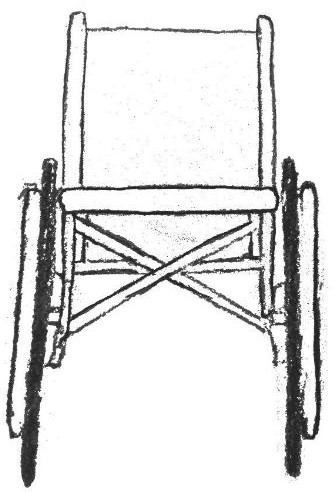
\includegraphics[height=10cm]{tires/wheelchair}
    \caption{A Standard Unmodified Wheelchair}
    \label{fig:tires-wheelchair}
\end{figure}

\subsection{Stakeholder and User Requirements}
The mountain bike tire subsystem addresses user and stakeholder needs by
improving the quality of life of the end user. The addition of mountain
bike tires extends the user's range of mobility. Locations that may have been
inaccessible with an unmodified wheelchair may become more accessible with the
mountain bike tires. In addition, caregivers will be able to maneuver the user more easily on rough
terrain, reducing the work required for simple tasks.

The addition of mountain bike tires to the wheels extends the life of the
wheels, and as a result, extends the life of the wheelchair. This directly
addresses client concerns of wheelchair life in variable terrain.

%The client also expressed concern with the rough terrain of Africa and how
%modern day wheelchairs were just not built to withstand the harsh conditions.
%This subsystem will directly solve this problem. By using an already available
%tire that was designed for the unpredictable landscape as:
%
%\begin{itemize}
%    \item The lifespan of the wheel is also expanded. Replacements don’t have to come as
%        often, therefore distributors don’t have to travel as often to pass out new
%        parts.
%    \item Manufacturers will not have to create new parts out of raw materials, reducing
%        waste.
%\end{itemize}

\subsection{Installation Manual}
In addition to the illustrated installation instructions, the FoWheel team
provides the following instructions. The installation process takes roughly 30
minutes to 2 hours.

\textbf{To install the bike tires:}

\begin{enumerate}
    \item Find bike tires that are slightly larger than the wheelchair wheels. Before
        you take the wheels off of the old bike, make sure the bike tires are
        deflated.
    \item Figure \ref{fig:tires-dimen} shows the diameter of the bike tire is 66
        $cm$ and the width is 5 $cm$, while the wheelchair wheel has a diameter
        of 61 $cm$ with a width of 3.05 $cm$.
    \item The best way to put the tires on the wheelchair is to first unscrew the
        wheels and separate them from the wheelchair. To do this, remove the center
        cap on the wheelchair wheels to access the hex bolt as shown in
        Figure \ref{fig:tires-step2}
    \item Use an adjustable wrench to remove the hex bolt.
    \item Figure \ref{fig:tires-step4} shows the correct side the tire should be
        placed on the wheelchair wheel. It is easier to put the tire onto the
        wheelchair wheel starting on the side of the wheel opposite of the handle bars.
        If the tire is a snug fit, make sure to use a solid piece of metal like a
        screwdriver to carefully stretch the tires onto the wheels.
    \item Afterwards, screw the wheels back onto the chair.
\end{enumerate}

To remove the bike tires, follow the instructions in reverse.

\begin{figure}[H]
    \centering
    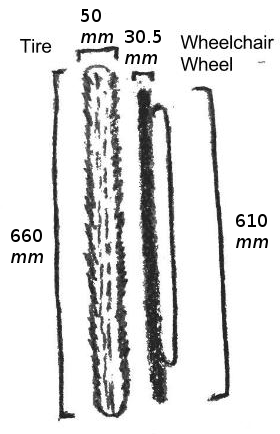
\includegraphics[height=9cm]{tires/dimen}
    \caption{Standard Wheel Sizes and Dimensions}
    \label{fig:tires-dimen}
\end{figure}

\begin{figure}[H]
    \centering
    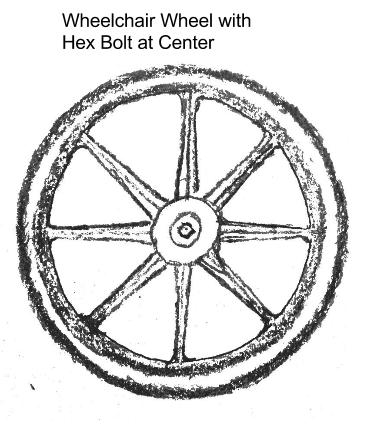
\includegraphics[height=9cm]{tires/wheel}
    \caption{Detaching wheels from wheelchair by removing hex bolt}
    \label{fig:tires-step2}
\end{figure}

\begin{figure}[H]
    \centering
    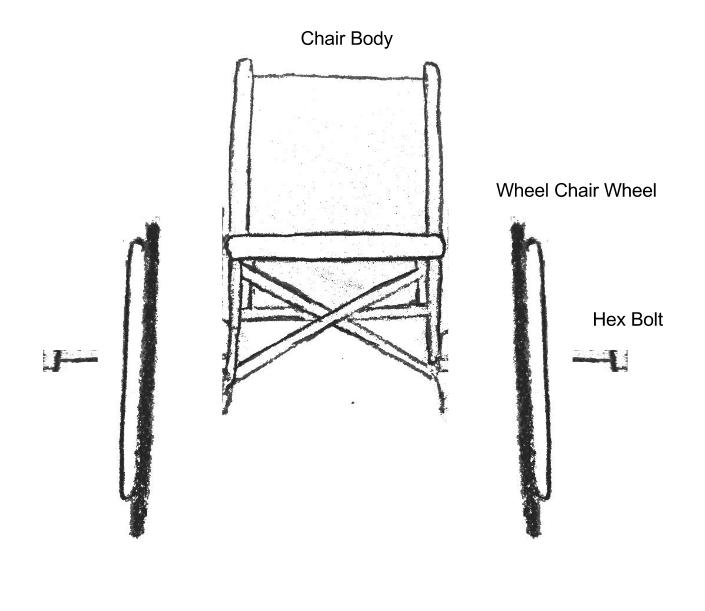
\includegraphics[height=9cm]{tires/detach}
    \caption{Removing both wheels from wheelchair body}
    \label{fig:tires-step3}
\end{figure}

\begin{figure}[H]
    \centering
    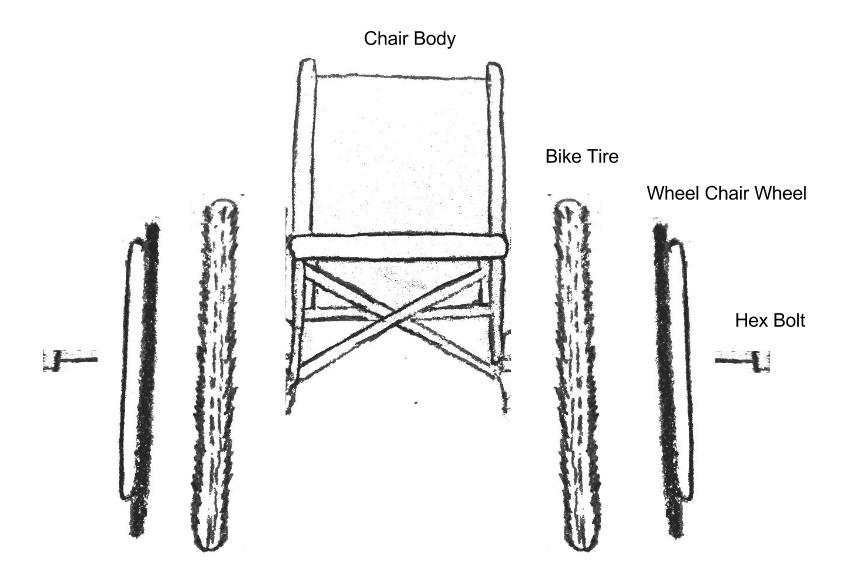
\includegraphics[height=9cm]{tires/insert}
    \caption{Inserting bike tires on the inside of the wheels}
    \label{fig:tires-step4}
\end{figure}

\begin{figure}[H]
    \centering
    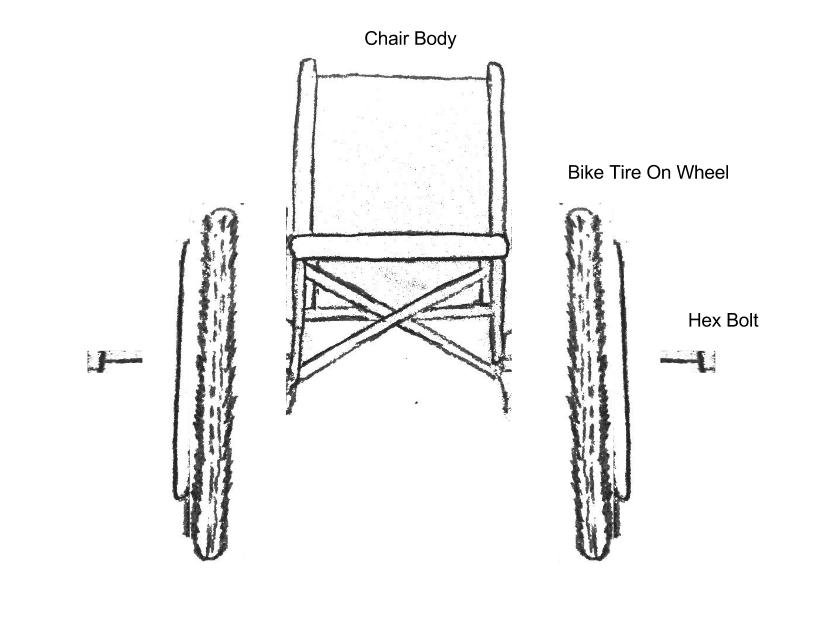
\includegraphics[height=10cm]{tires/wrap}
    \caption{Wrapping tires over the wheels}
    \label{fig:tires-step5}
\end{figure}

\begin{figure}[H]
    \centering
    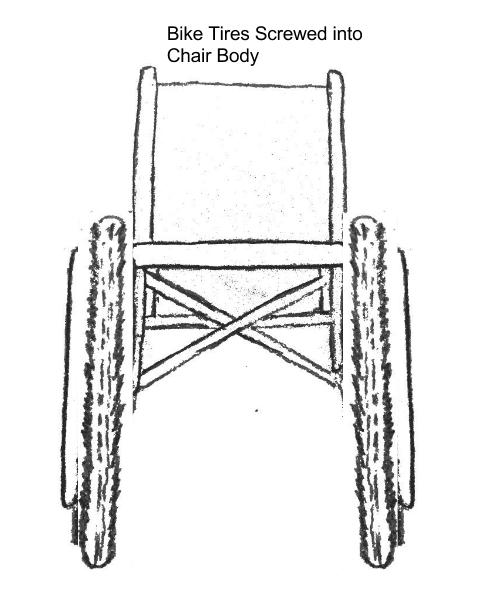
\includegraphics[height=10cm]{tires/replace}
    \caption{Replacing the hex bolt and installing the wheels}
    \label{fig:tires-step6}
\end{figure}

\subsection{Materials}
The following materials are required to install the mountain bike tire treads:

\begin{itemize}
    \item Mountain Bike Tire Treads
    \item Adjusting Wrench - For loosening and tightening any size hex bolt from the wheelchair
        wheels.
    \item Screwdriver - Used to edge the tire onto the wheelchair wheel.
\end{itemize}

\subsection{Cost Analysis}
Table~\ref{tbl:tire-cost} shows the cost of the parts for this subsystem, as
well as the estimated total cost of the subsystem. The table also
provides the preferred dimensions for the mountain bike tires.

\begin{table}[H]
    \centering
    \caption{Cost Analysis for Mountain Bike Tire Tread Installation}
    \label{tbl:tire-cost}
    \begin{tabular}{ l l }
        Description & Estimated Cost \\
        \hline \\[-1.2em]
        \parbox{6cm}{Mountain Bike Tire Treads \\ \emph{66 $cm$ diameter, 5
        $cm$ width}} & 12.00 USD\cite{tirecost} \\[0.6em]
        Labor Costs & 0.00 USD\footnotemark[1]\\
        \hline
        Estimated Subsystem Cost & 12.00 USD
    \end{tabular}
\end{table}
\footnotetext[1]{Assuming volunteer labor}

The intention of our design is to use recycled bicycle parts rather than
purchasing new parts. However, Table~\ref{tbl:tire-cost} shows the cost of the
parts should they be unavailable.

\subsection{Calculations}
%\begin{center}
%    \begin{align*}
%        mass_{bike tire} &= 240 g \\
%        mass_{wheelchair} &\approx 16 kg \\
%        mass_{user} &\approx 60 kg \\
%    \end{align*}
%\end{center}

The amount of surface area touching the ground can be calculated:

\textbf{Standard Wheelchair Wheels}
\begin{center}
    \begin{align*}
        width_{wheel} &= 3.05 \, cm \\
        r_{wheel} &= 61 \, cm \\
        {S.A.}_{wheel} = 2\pi \times r_{wheel} \times width_{wheel} &= 1160 \, cm^2 \\
    \end{align*}
\end{center}

\clearpage
\textbf{Mountain Bike Tires Added}
\begin{center}
    \begin{align*}
        width_{tire} &= 5.0 \, cm \\
        r_{tire} &= 66 \, cm \\
        {S.A.}_{tire} = 2\pi \times r_{tire} \times width_{tire} &= 2073 \, cm^2 \\
    \end{align*}
\end{center}

With the retrofitted bike tires, there is nearly twice as much wheel surface
area now making contact with the ground giving the user twice as much more
stability and control over their wheelchair.

\subsection{Relations to the Other Subsystems}
As the seatbelt is installed within close proximity to the bike tires, the
seatbelt placement must not interfere with the wheels or the bike tires.
Additionally, as the bike tires provide a significant amount of additional
traction, the user may be more inclined to participate in potentially dangerous
activities. Additionally, the seatbelt must have the safety features to
accommodate for potentially dangerous activities.

Both the seatbelt and the cup holder provide storage area for items while the
user is operating the wheels.

%The bike tire retrofit is the main subsystem of the overall design proposal. It
%will consume the most amount of time to install. It will may also be the most
%expensive component of the design. The overall benefit will prove to outweigh
%the costs. The user is now free to explore more of his or her prospective area
%and can make more of a contribution to society. All other subsystems complement
%the bike tires in a way that will make riding the wheelchair more comfortable
%and safe:
%
%\begin{itemize}
%    \item Cup Holder – When using the bike tires, the user must have both hands available
%to maneuver the wheelchair. To the user’s convenience, a cup holder will be
%added so that the user can store items while moving the wheelchair. Providing a
%more comfortable ride.
%\item Seatbelt – The addition of the bike tires will present new challenges for the
%user. Rocky and inclined terrain can increase the chances of the user of
%falling out. By installing the seatbelt, the user is now safe in his or her
%chair and doesn’t have to worry about the possibility of further injury.
%\end{itemize}

\section{Seat Belt}
Many modern devices, like cars, in which a user is in motion, contain seat belts.
Seat belts are a proven method to protect a user's safety in
motion\cite{fedorowicz1985seat}. In the
unpredictable terrain of rural communities in Africa, a seatbelt can protect a
user from injury.

Our design implements a seatbelt not only to protect the user, but also to
assist the user in carrying larger objects in their lap. The seatbelt can strap
around these objects to allow the user to operate the wheels while concurrently
carrying items.
%An aspect of traction that reached out to our team was safety. By attaching
%bike tires to the wheelchair and allowing it to maneuver over rocky and
%inclined terrain brings rise to the possibility of added injury. When it comes
%to wheelchairs, safety must be of the utmost concern to prevent further and
%unnecessary injury to the user. Currently, most wheelchairs do not have a
%mechanism to brace oneself after braking at high speeds. Braking at high speeds
%over a short period of time would cause a jerking motion, which in turn, turns
%the wheelchair into a low-tech catapult. With these concerns in mind, the team
%has decided to implement a seatbelt. Used in cars, planes, trains, etc. today,
%why not in wheelchairs as well? In order to protect the most “at risk” people
%of the world, we must take the proper precautions. Consisting of only rope or
%some other fibrous material, the seatbelt would act as a barrier to prevent the
%user from falling out of the chair. A secondary use of the seatbelt is that it
%can help secure large bulky items to the user if he or she needed to carry such
%an item. It would leave the user’s hands free to move the wheelchair around. It
%can easily be installed, considering the limited resources available. The
%modification from the current wheelchair would simply be that a rope would be
%anchored to the body of the wheelchair and go across the body of the user.
%Whether it be from braking at high speeds or a simple incline, the user would
%remain snug in the wheelchair.

\subsection{Stakeholder and User Requirements}
The seatbelt helps reduce risk of injury when using the wheelchair. The wheelchair user can safely maneuver
through inclines and rocky terrain without slipping out of the seat.
During our user empathy tests, we found getting in and out of the
wheelchair to be a difficult task. With the seatbelt:

\begin{itemize}
    \item The wheelchair user will not fall out of the chair and
have to lift themselves back, saving time and energy.
\item Caregivers will be able to move the wheelchair without injuring the user.
\item Locals responsible for installing the seatbelt can easily be taught the
strongest types of knots in order to ensure maximum safety.
\item The seatbelt is a lightweight addition with all materials available
    locally, removing extra weight for distributors.
%\item Distributors don’t have to fret over extra weight when transporting the rope
%because the locals are sure to have some at hand.
%\item Manufacturers have no extra work for the same reason. Locals are sure to have
%all the items needed, just lying around in their villages/cities/etc.
\end{itemize}

%With almost no extra cost to Crutches4Africa, this subsystem provides a cost
%effective solution and that benefits all stakeholders/users.

\subsection{Installation Manual}
In addition to our illustrated instructions, the FoWheel team provides the
following installation instructions. The installation process will take
approximately 5 minutes.

\textbf{To install the seatbelt:}

\begin{enumerate}
    \item Measure out two pieces of rope or similar material, one of 120 $cm$,
        and another of 30 $cm$.
    \item Taking the shorter piece, tie two tight loops on both ends.
    \item Take one loop, place the loop over one of the handles of the
        wheelchair.
    \item Taking the longer piece, attach it to the opposite side of the
        wheelchair.
    \item Take the loose end of the long rope and pull the rope through the other loop.
\end{enumerate}

\begin{figure}[H]
    \centering
    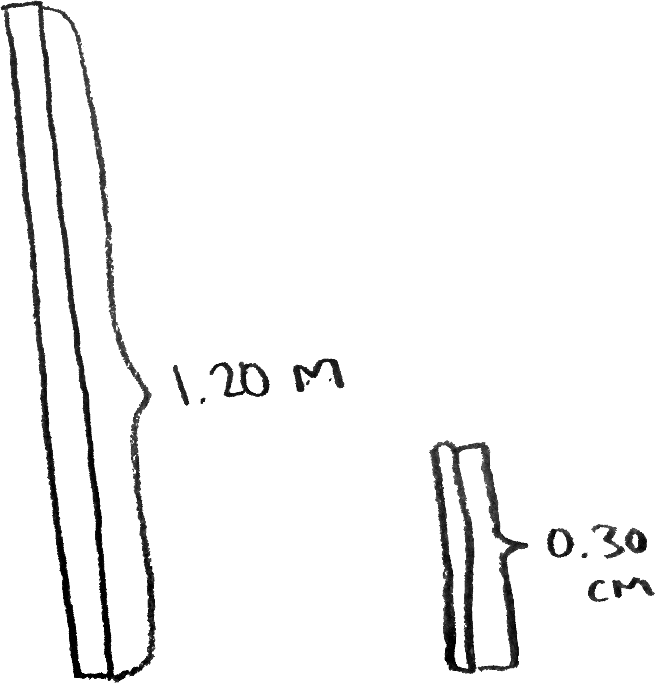
\includegraphics[height=6cm]{ropesizes}
    \caption{Rope Dimensions for the Seatbelt}
\end{figure}

\begin{figure}[H]
    \centering
    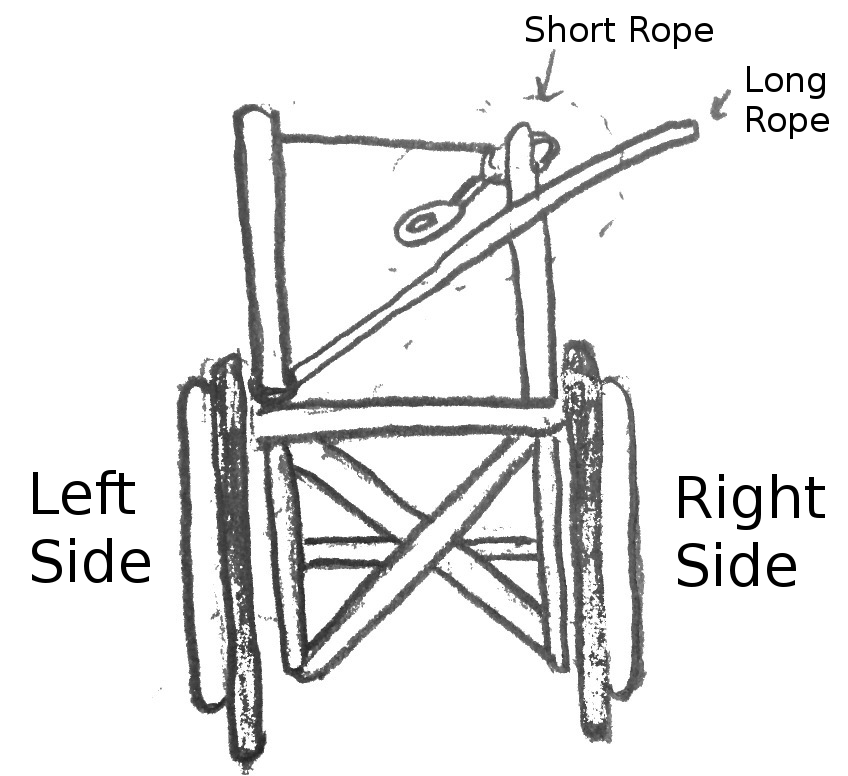
\includegraphics[height=9cm]{sbasm}
    \caption{Seatbelt Assembly}
\end{figure}

\subsection{Materials}

In order to install the seatbelt, the following materials are required:

\begin{itemize}
\item Rope or similar material – To use as the seatbelt
\item Scissors or a knife – To cut the rope with
\item Measuring tape – To get precise rope measurements
\end{itemize}
Additionally, fastening points on the wheelchair for the rope can be attached
will be required to install a seatbelt.

\subsection{Cost Analysis}

Table~\ref{tbl:seatbelt-cost} on the next page shows the cost estimation for the installation of
a seatbelt on a wheelchair.

\begin{table}[H]
    \centering
    \caption{Cost Analysis for the Seatbelt}
    \label{tbl:seatbelt-cost}
    \begin{tabular}{l c l}
        Description & Quantity & Estimated Cost \\
        \hline
        \\[-1.2em]
        Seatbelt & \parbox{4cm}{120 $cm$ long rope \\ 30 $cm$ short rope} &
        0.70 USD \\
        Labor costs & 5 $min$ & 0.00 USD\footnotemark[1] \\
        \hline
        \multicolumn{2}{r}{Estimated cost per chair} & 0.70 USD
    \end{tabular}
\end{table}
\footnotetext[1]{Assuming volunteer labor}

\subsection{Relations to the Other Subsystems}
The addition of the bike tires allow for the user to travel over
rocky or uneven terrain. By travelling over such dangerous terrain, a seatbelt
is necessary to ensure the user's safety.

\section{Cup Holder}
One of the challenges a wheelchair user faces is carrying objects while having
to propel the chair. In order to solve this problem, we have installed a
carrying mechanism: a cup holder. This subsystem consists of a foam cup holder
attached to the top of the arm of the wheelchair with duct tape. The cup holder allows the
user to carry small objects without the need to use their hands, freeing them
to spin the drive wheels.

\subsection{Technical Specifications}
This subsystem must be attached firmly so the cup holder does not slide sideways and end up
under the chair arm. The cup holder is created using a foam cup holder, scissors, and a
roll of tape (duct tape is used here). The scissors are used to cut a slit in
two opposite sides of the cup holder, slits long enough to fit the tape
through. A portion of the tape should be folded over upon itself so the tape does
not stick to the cup holder while attached. The tape is then pushed through
the cup holder so the folded over portion sticks out the opposite end and the
sticky side is still on the original side. The cup holder is then taped tightly
to either arm of the chair.

\begin{table}[H]
    \centering
    \label{tbl:cupholder-cost}
    \caption{Cup Holder Cost Analysis}
    \begin{longtable}{l c l}
        Description & Quantity & Estimated Cost \\
        \hline
        Foam Cup Holder & 1 & 0.27 -- 0.52 USD\cite{cost-cupholder} \\
        Scissors & 1 per worker & Negligible \\
        Duct Tape of $\leq 50$ $mm$ width & $\sim 250$ $mm$ & 0.01
        USD\footnotemark[1] \\
        Labor Cost & $\sim 1$ $min$ & 0.00 USD\footnotemark[2] \\
        \hline
        \multicolumn{2}{r}{Estimated cost per chair} & 0.28 -- 0.53 USD
    \end{longtable}
\end{table}
\footnotetext[1]{The labor cost per chair is negligible as this will be done by volunteers.}
\footnotetext[2]{The cost of tape per chair was determined by finding the
    cost of a roll of 18288~$mm$ of duct tape
    ($\sim$3.50~USD\cite{cost-ducttape}) and applying
this to an estimated length per chair. This length was intentionally overestimated.}
\subsection{Stakeholder and User Requirements}
This subsystem addresses the concern of users ability to carry objects. It
gives them a convenient place to carry small objects.

During the user empathy activities and the client's presentation, this
topic appeared often. People in Africa are expected to provide for
themselves as much as possible, and being able to carry necessary objects
or fluids reliably is a step in that direction. Often, wheelchair users
place objects in their laps to carry them. They cannot usually grip these
objects, as they must use their arms to move the wheelchair. This
is especially common with very large or very small objects. The cup holder
addresses the problem of carrying small objects.

\subsection{Relations to the Other Subsystems}
The cup holder works with the seat belt to allow for carrying objects. While
the cup holder allows the user to carry small objects, the seat belt allows the
user to carry larger objects. Together, these subsystems solve the problem as
completely as possible.

\begin{figure}[H]
    \label{fig:cupholderasm}
    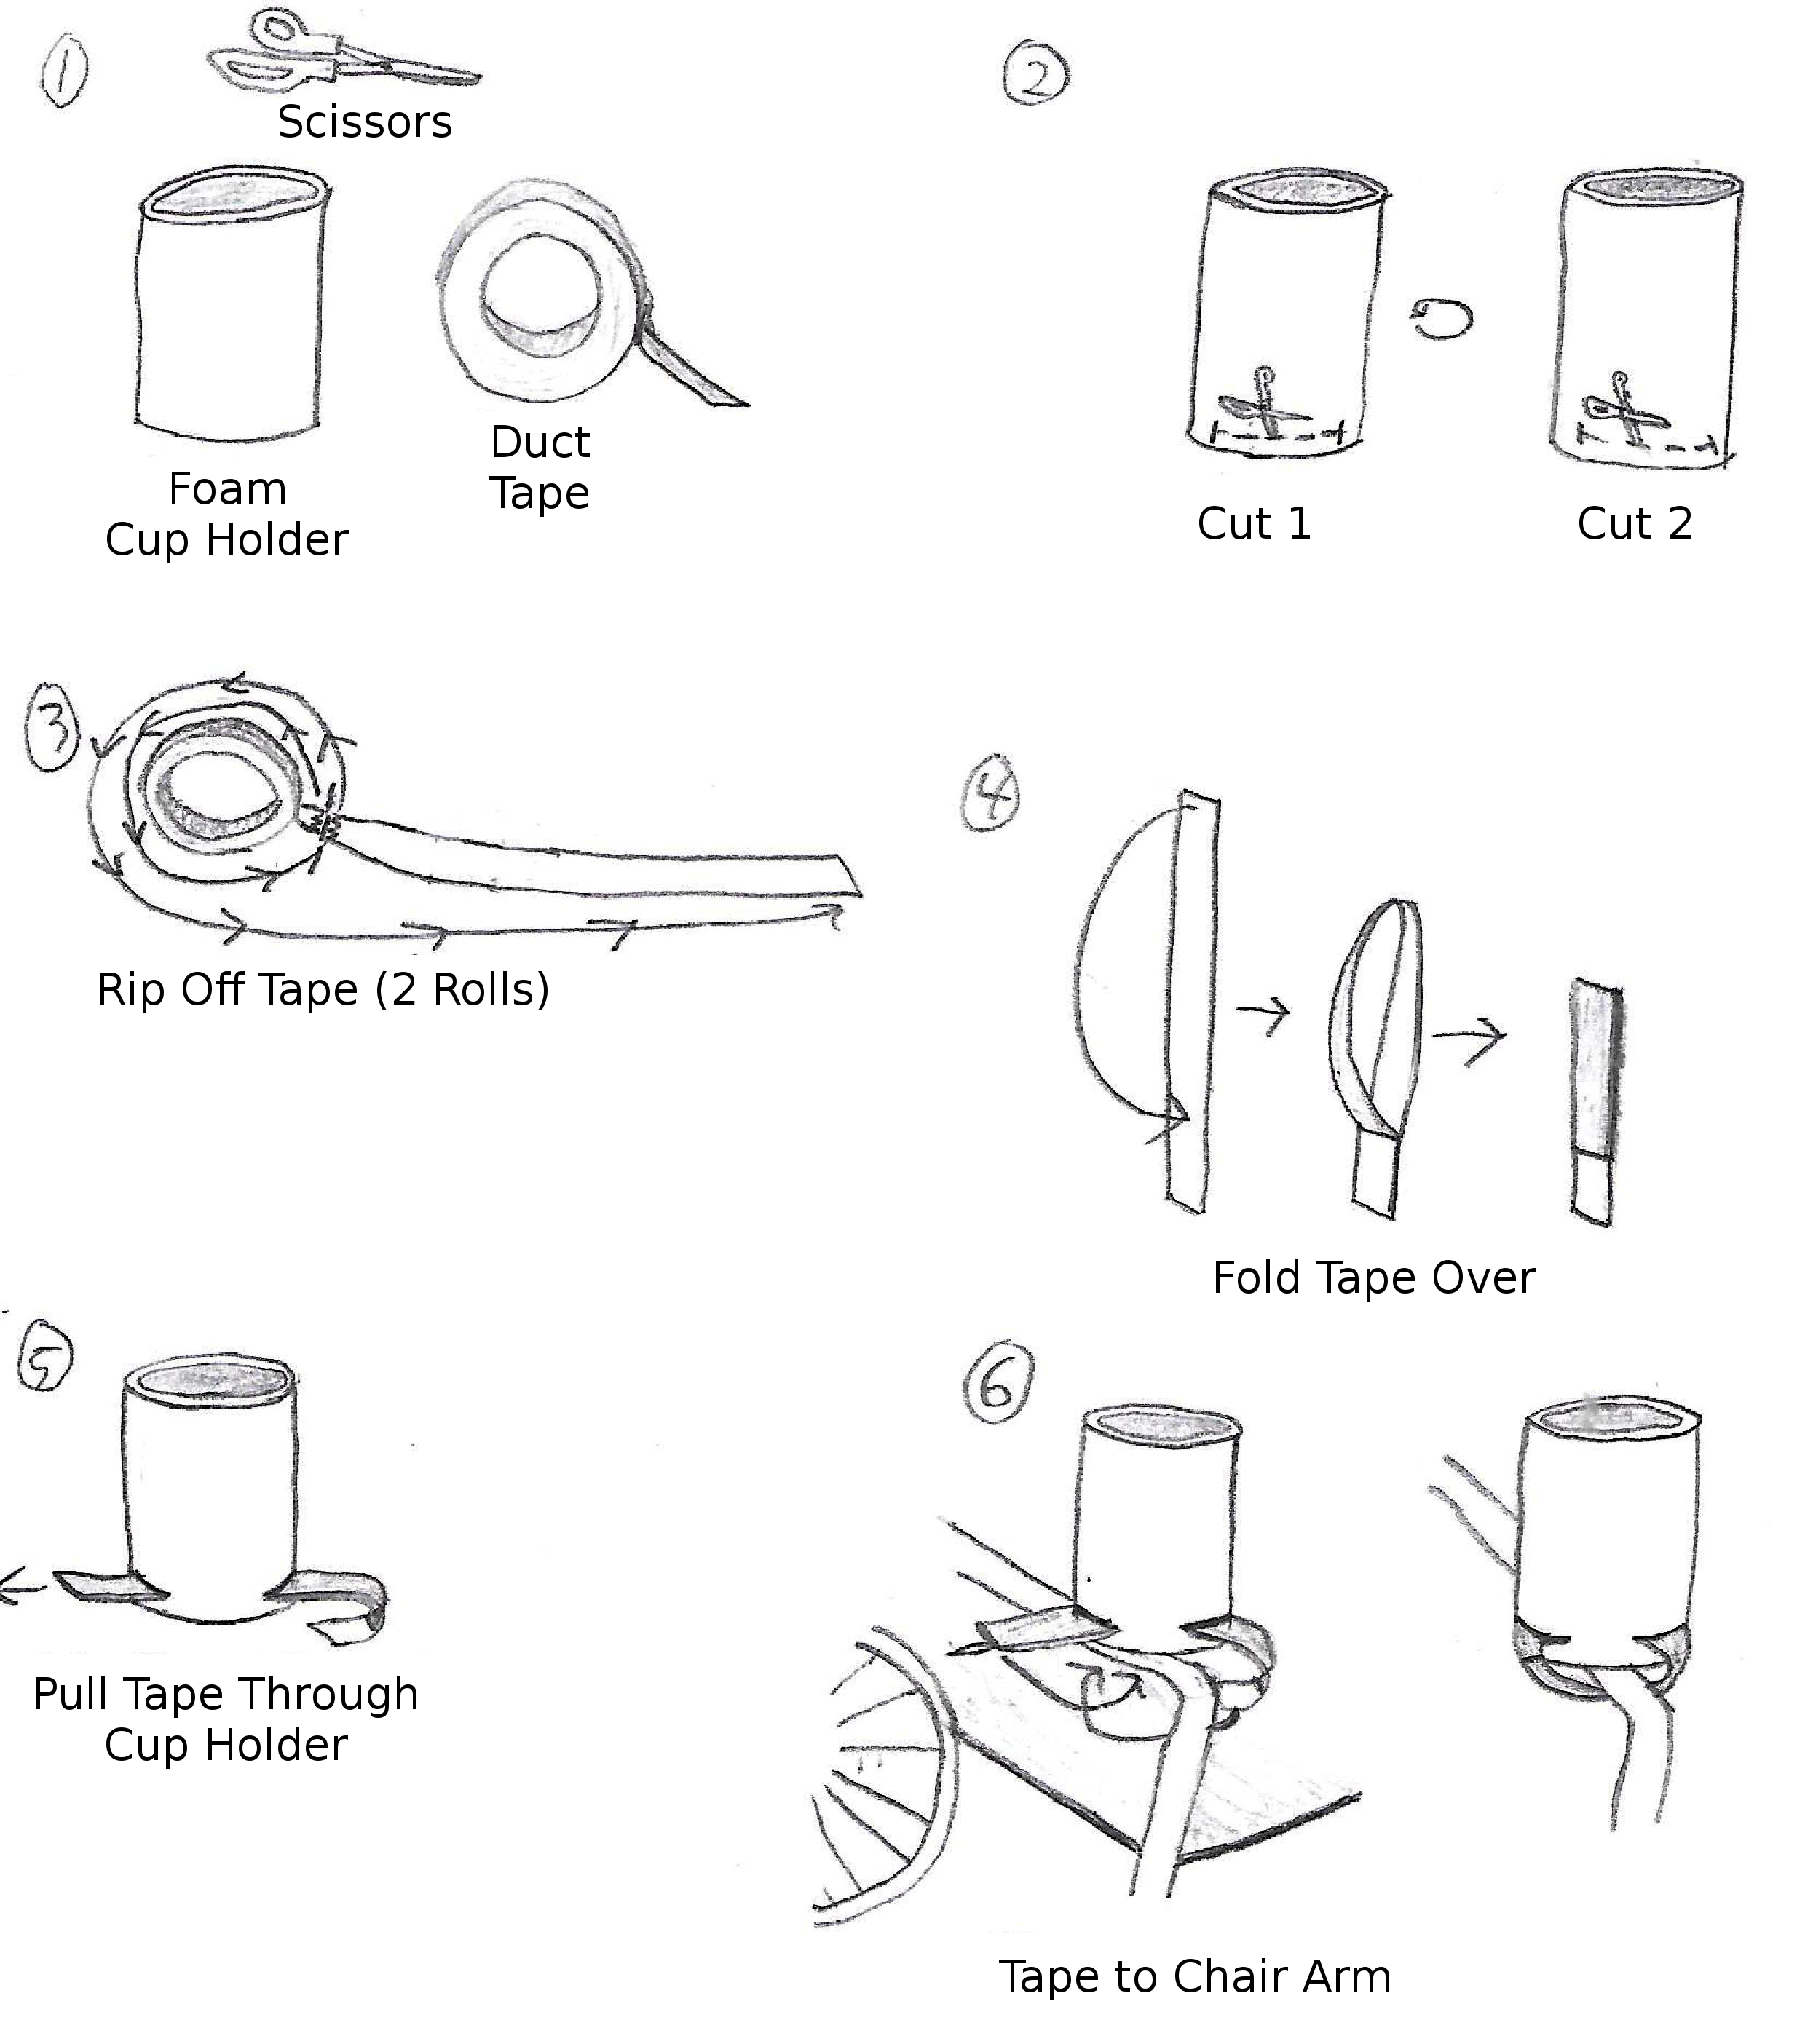
\includegraphics[width=\textwidth]{cupholderasm}
    \caption{Illustrated Assembly for the Cup Holder}
\end{figure}

\begin{figure}[H]
    \centering
    \label{fig:cupholder-solid}
    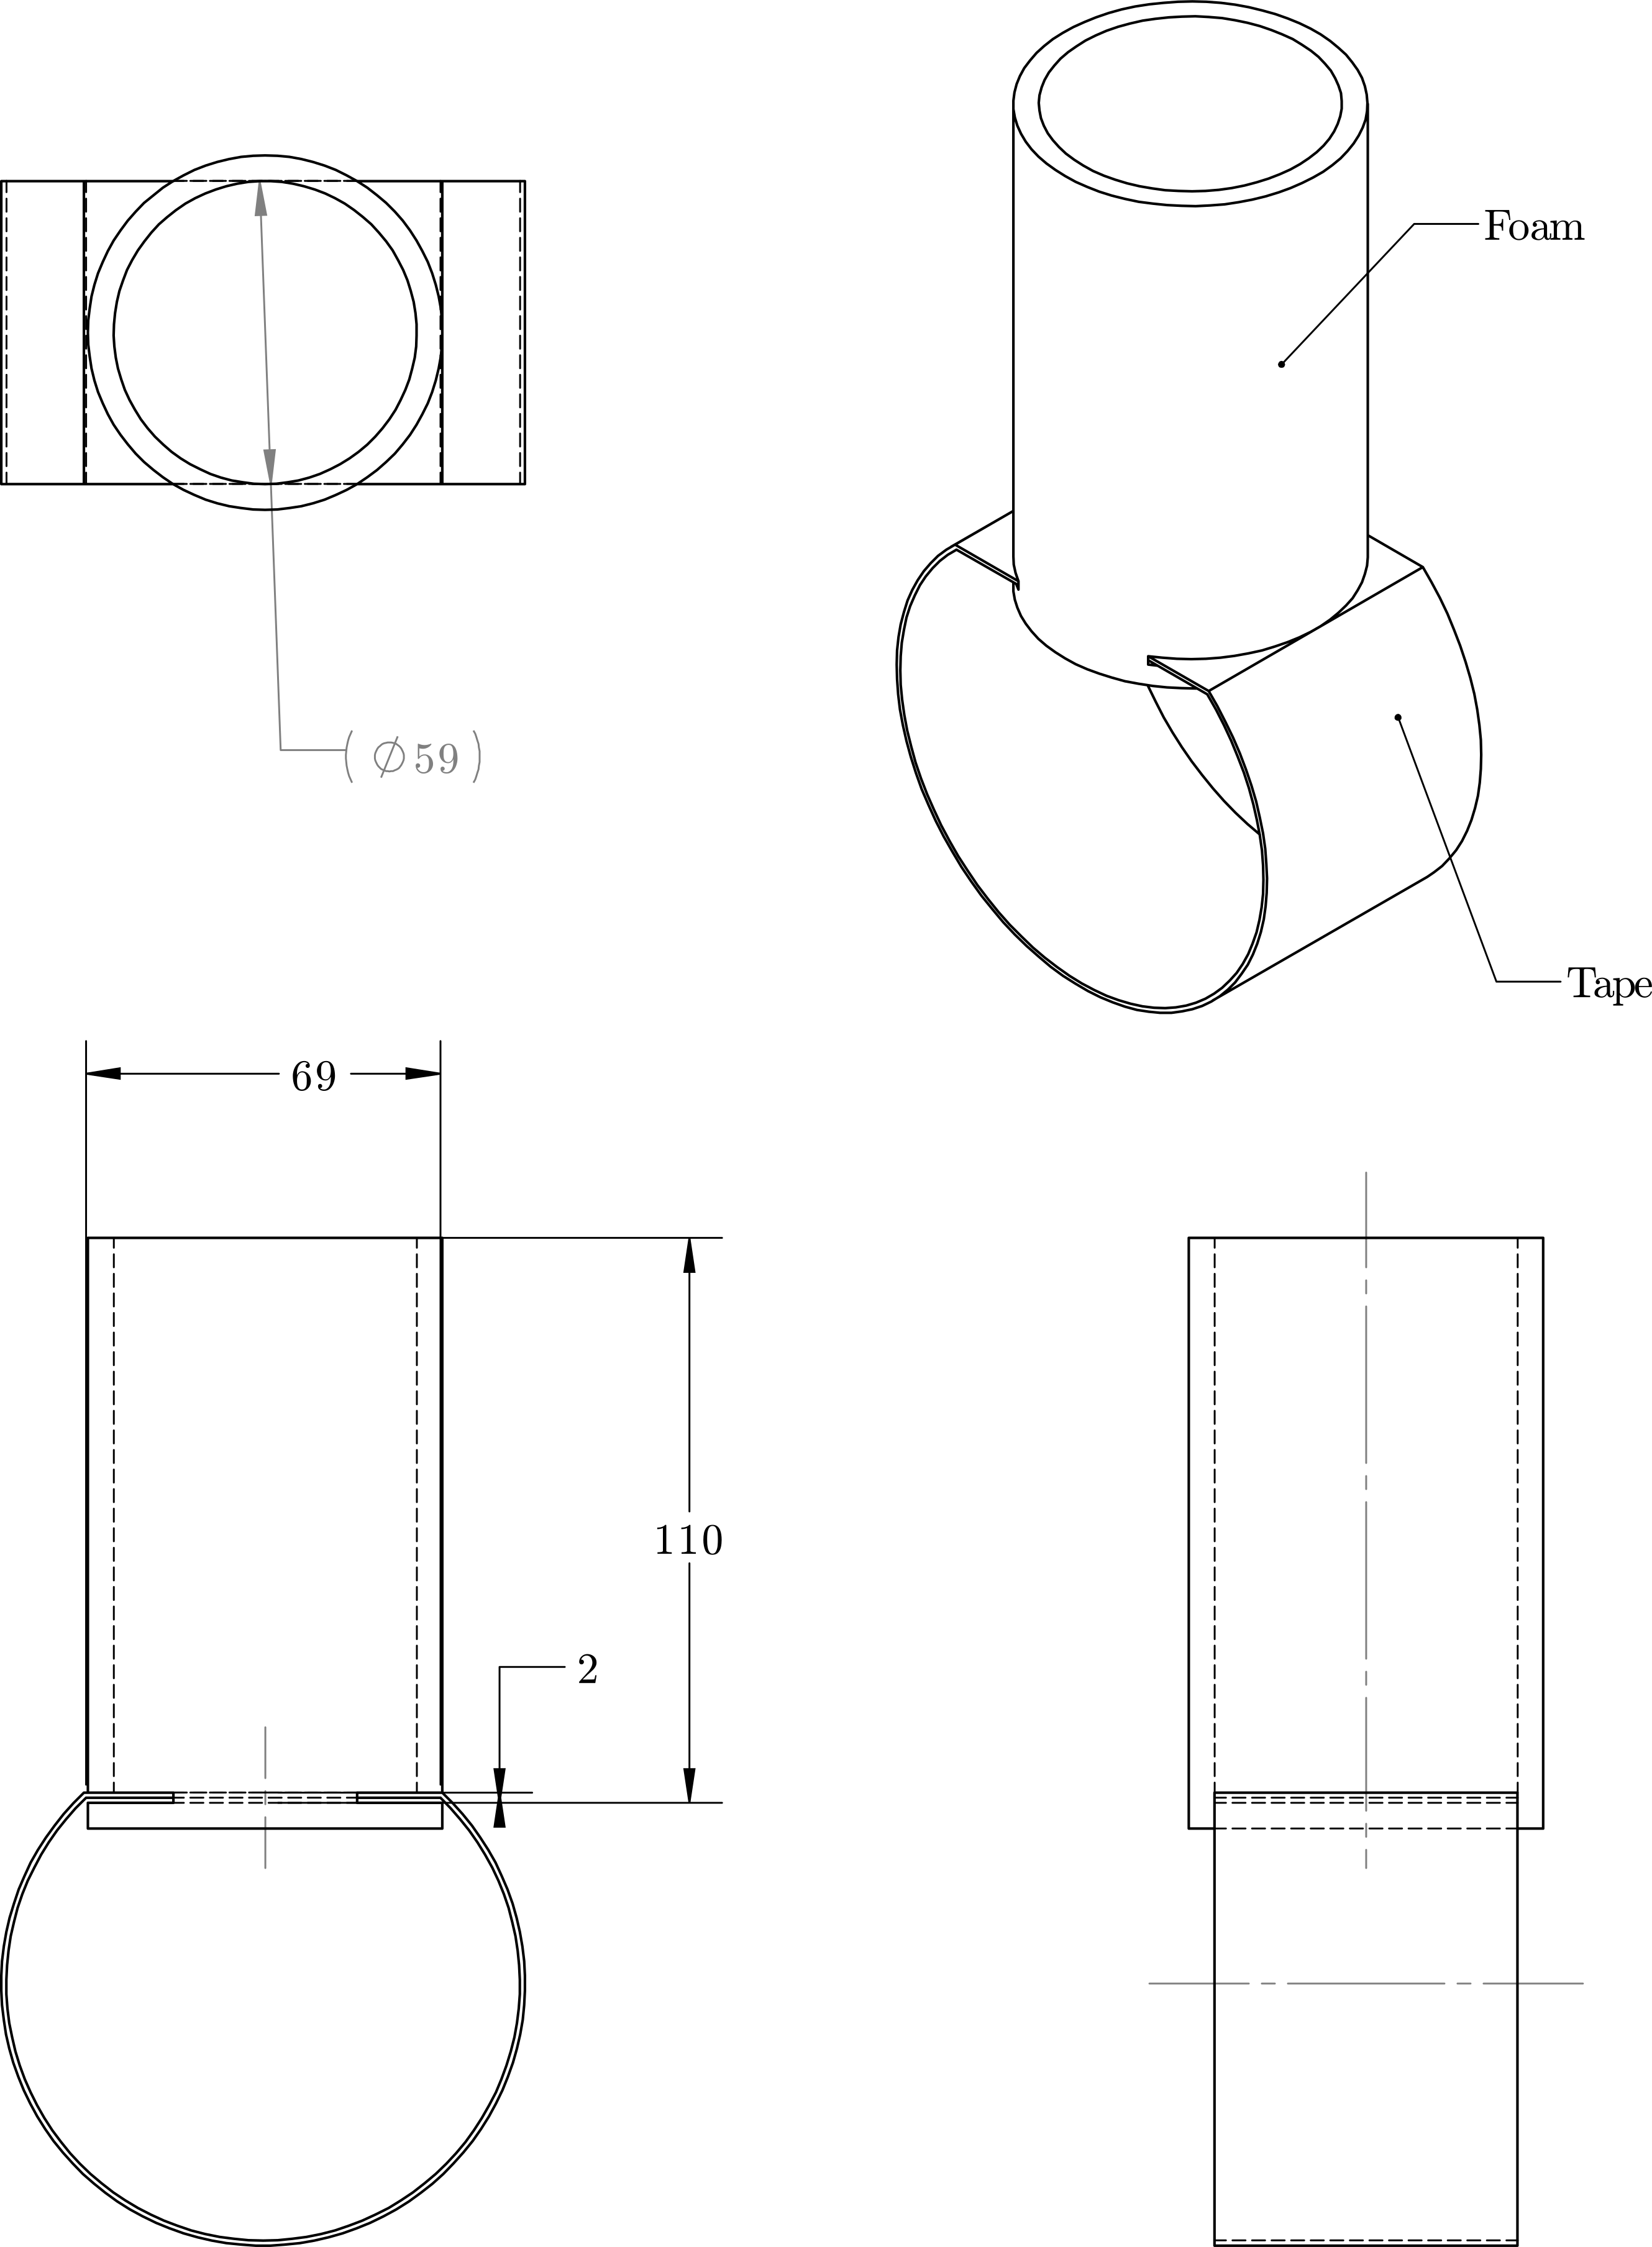
\includegraphics[width=0.9\textwidth]{cupholder-solid}
    \caption[Cupholder 3D Sketch with Dimensions]{Cupholder 3D Sketch with Dimensions \\ Dimensions calculated using
    standard can sizes\cite{dimen-cansize} using large tolerance}
\end{figure}

%\begin{center}
%    \begin{tikzpicture}
%        \draw[help lines,step=2mm] (-1,-0.1); %grid (4,1.1);
%        % Draw the Ford circles
%        \tikzmath{FordCircles(-.9,3.9,8);}
%    \end{tikzpicture}
%\end{center}

\printbibliography
\addcontentsline{toc}{chapter}{Bibliography}

\end{document}
